\documentclass[11pt]{article}
 \renewcommand{\familydefault}{\sfdefault}

\usepackage{listings}
\usepackage{xcolor}
\lstset{
    language=SQL, % Set the language to SQL
    basicstyle=\ttfamily\color{black}, % Regular font style
    commentstyle=\color{green!60!black}, % Set the color for comments
    keywordstyle=\bfseries\color{blue}, % Bold and color for keywords
    stringstyle=\color{orange}, % Set the color for strings
}

\usepackage{tabularx}
\usepackage{changepage}
\usepackage{amsfonts}
\usepackage{float}
\usepackage{amsmath}
\usepackage{graphicx}
\usepackage{hyperref}
\usepackage{caption}
\usepackage{fancyhdr}
\usepackage{geometry}
	\geometry{height=24 cm}
	\geometry{left=2.5 cm}
	\geometry{right=2.5 cm}
	\geometry{top=2 cm}
	\geometry{headheight=1 cm}

\setcounter{secnumdepth}{2}
\linespread{1}
\renewcommand{\labelitemi}{-}
\pagestyle{empty}


\begin{document}

\begin{center}
	\huge{\textbf{ECloth Mountain}}
\end{center}

\section{Abstract}
"ECloth Mountain" è un'azienda speccializzata nella vendita di abbigliamento 
tecnico da montagna, ha appena aperto il proprio sito di e-commerce e ha
commissionato il proprio database. \\
Dal sito di "ECloth Mountain" è possibile registrarsi e creare un account, per
salvare i propri dati e per poter effettuare acquisti. Inoltre è possibile
creare varie liste di prodotti, per poterli salvare e visualizzare in un secondo
momento. \\
L'utente per registrarsi deve inserire i propri dati personali, mentre
l'indirizzo e il metodo di pagamento non sono obbligatori. L'indirizzo e il
metodo di pagamento sono necessari al momento dell'acquisto, ma l'utente può 
decidere di non salvarli. L'utente attraverso il proprio account può rivedere 
gli acquisti effettuati e le liste di prodotti salvate.

\section{Analisi dei requisiti}

\subsection{Descrizione testuale}

Nella base di dati sono presenti i dati degli \textbf{utenti}, che si registrano
sul sito per effettuare gli acquisti. Di ogni utente sono noti: 

\begin{itemize}
	\item nome
	\item cognome
	\item email
	\item password
\end{itemize}

Ogni utente può memorizzare i dati di una \textbf{carta di credito}. Di ogni
carta di credito sono noti:

\begin{itemize}
	\item numero della carta
	\item intestatario della carta
	\item data di scadenza
	\item codice di sicurezza (CVV)
\end{itemize}

Ogni utente può memorizzare i dati di vari indirizzi di spedizione. Di ogni
\textbf{indirizzo} sono noti:

\begin{itemize}
	\item via
	\item numero civico
	\item città
	\item CAP
	\item stato
\end{itemize}

Ogni utente può avere diversi carrelli. Di ogni \textbf{carrello} sono noti:

\begin{itemize}
	\item nome del carrello
	\item costo totale
	\item data di creazione
	\item data di ultima modifica
	\item prodotti contenuti
\end{itemize}

Ogni utente può effettuare un \textbf{ordine}, effettuando il \textit{checkout}
del carrello desiderato. Di ogni ordine sono noti:

\begin{itemize}
	\item numero dell'ordine
	\item costo totale
	\item data di creazione
	\item data di ultima modifica
	\item prodotti contenuti
	\item provider del pagamento
	\item status dell'ordine
	\item indirizzo di spedizione
\end{itemize}

I pagamenti sono gestiti mediante un provider esterno, che si occupa di
effettuare il pagamento e di notificare il sito di "ECloth Mountain" del
risultato dell'operazione. \\
Gli utenti possono acquistare dei prodotti, presenti sul sito. Di ogni
\textbf{prodotto} sono noti:

\begin{itemize}
	\item nome
	\item descrizione
	\item prezzo
	\item quantità
	\item tag
\end{itemize}

Non è possibile acquistare un prodotto se la quantità disponibile è minore di
quella richiesta. 

\begin{table}[H]
	\centering
	\begin{tabularx}{\textwidth}{|l|X|l|}
		\hline
		\textbf{Termine} & \textbf{Descrizione} & \textbf{Collegamenti} \\
		\hline
		Utente & Persona che si registra sul sito & Carta di credito,
		Lista, Indirizzo \\
		\hline
		Carta di credito & Carta di credito di un utente & Utente \\
		\hline
		Indirizzo & Indirizzo di spedizione di un utente & Utente,
		Ordine \\
		\hline
		Lista & Lista di prodotti, con relativo costo totale & Utente,
		Prodotto \\
		\hline
		Carrello & Lista con un nome & Entità figlia di Lista \\
		\hline
		Ordine & Lista con un identificativo e i dettagli di pagamento
		& Indirizzo, Entità figlia di Lista \\
		\hline
		Prodotto & Prodotto in vendita sul sito & Lista, Categoria \\
		\hline
		Categoria & Categoria di prodotti & Prodotto \\
		\hline
	\end{tabularx}
	\caption{Glossario dei termini}
\end{table}

\begin{table}[H]
	\centering
	\begin{tabular}{|l|l|l|}
		\hline
		\textbf{Operazione} & \textbf{Tipo} & \textbf{Frequenza} \\
		\hline
		Inserimento di un nuovo Utente & U & 1 volta al giorno \\
		\hline
		Inserimento di una Carta di Credito & U & 5 volte al giorno \\
		\hline
		Inserimento di un Indirizzo & U & 20 volte al giorno \\
		\hline
		Inserimento di un nuovo Carrello & U & 20 volte al giorno \\
		\hline
		Cancellazione di un Carrello & U & 10 volte al giorno \\
		\hline
		Visione di un Carrello & U & 100 volte al giorno \\
		\hline
		Aggiungi un Prodotto al Carrello & U & 100 volte al giorno \\
		\hline
		Rimuovi un Prodotto dal Carrello & U & 90 volte al giorno \\
		\hline
		Inserimento di un nuovo Ordine & U & 10 volte al giorno \\
		\hline
		Cancellazione di un Ordine & U & 1 volte al giorno \\
		\hline
		Visione di un Ordine & U & 10 volte al giorno \\
		\hline
		Inserimento di un nuovo Prodotto & B & 10 volte alla settimana \\
		\hline
		Calcolare il guadagno mensile & B & 1 volta al mese \\
		\hline
		Calcolare il guadagno quotidiano & B & 1 volta al giorno \\
		\hline
	\end{tabular}
	\caption{Operazioni}
\end{table}

\section{Progettazione concettuale}

\renewcommand{\labelitemi}{\textbullet}
\subsection{Lista delle entità}
\begin{itemize}
	\item Utente
		\begin{itemize}
			\item \underline{email} VARCHAR(255) PK NOT NULL
			\item password VARCHAR(255) NOT NULL
			\item nome VARCHAR(255) NOT NULL
			\item cognome VARCHAR(255) NOT NULL
		\end{itemize}

	\item Carta di credito
		\begin{itemize}
			\item \underline{numero} VARCHAR(16) PK NOT NULL
			\item intestatario VARCHAR(255) NOT NULL
			\item scadenza DATE NOT NULL
			\item cvv INT NOT NULL
		\end{itemize}

	\item Indirizzo
		\begin{itemize}
			\item \underline{via} VARCHAR(255) PK NOT NULL
			\item \underline{numero} PK INT NOT NULL
			\item \underline{cap} VARCHAR(5) PK NOT NULL
			\item citta VARCHAR(255) NOT NULL
			\item stato VARCHAR(255) NOT NULL
		\end{itemize}

	\item Lista
		\begin{itemize}
			\item \underline{id utente} INT PK NOT NULL
			\item \underline{data creazione} DATE PK NOT NULL
			\item data modifica DATE NOT NULL
			\item costo totale FLOAT NOT NULL
		\end{itemize}

		\begin{adjustwidth}{2em}{0pt}

			L'entità Lista si specializza in due sottocategorie con una 
			generalizzazione totale:

			\renewcommand{\labelitemii}{\textbullet}
			\renewcommand{\labelitemiii}{-}
			\renewcommand{\labelitemiv}{$\square$}


			\begin{itemize}
				\item Carrello
					\begin{itemize}
						\item nome VARCHAR(255) NOT NULL
					\end{itemize}

				\item Ordine
					\begin{itemize}
						\item numero INT NOT NULL

						\item dettagli pagamento: attributo composto:
							\begin{itemize}
								\item provider VARCHAR(255) NOT NULL
								\item status VARCHAR(255) NOT NULL
							\end{itemize}

					\end{itemize}
			\end{itemize}

		\end{adjustwidth}

	\item Prodotto
		\begin{itemize}
			\item \underline{nome} VARCHAR(255) PK NOT NULL
			\item \underline{tag} VARCHAR(255) PK NOT NULL
			\item descrizione VARCHAR(255)
			\item prezzo FLOAT NOT NULL
			\item quantità INT NOT NULL
		\end{itemize}

	\item Categoria
		\begin{itemize}
			\item \underline{nome} VARCHAR(255) PK NOT NULL
			\item descrizione VARCHAR(255)
		\end{itemize}
\end{itemize}

\begin{table}[H]
	\centering
	\begin{tabularx}{\textwidth}{|l|X|X|l|}
		\hline 
		\textbf{Relazione} & \textbf{Entità coinvolte} & \textbf{Descrizione} &
		\textbf{Attributi} \\
		\hline
		Metodo pagamento & Carta di credito (1, 1), Utente (0, 1) & Un utente
		può avere al più una carta di credito, una carta di credito si riferisce
		ad un solo cliente & Nessuno \\
		\hline
		Indirizzo spedizione & Indirizzo (0, N), Utente (0, N) & Un utente può
		avere più indirizzi di spedizione, o non averne uno affatto. Un
		indirizzo può essere associato a più clienti e può non avere nessun
		cliente & Nessuno \\
		\hline
		& Lista (1, 1), Utente (0, N) & Un utente può avere più liste, o non
		averne affatto. Una lista si riferisce ad un utente & Nessuno \\
		\hline
		Contenuto & Lista (0, N), Prodotto (0, N) & Una lista può contenere più
		prodotti, un prodotto può essere contenuto in più liste & quantità INT
		$>$ 0 \\
		\hline
		Spedizione & Ordine (1, 1), Indirizzo (0, N) & Un ordine può essere
		spedito ad un solo indirizzo. Un indirizzo può essere associato a più
		ordini & Nessuno \\
		\hline
		Tag & Prodotto (1, 1), Categoria (0, N) & Un prodotto appartiene ad una
		categoria, una categoria può avere più prodotti & Nessuno \\
		\hline
	\end{tabularx}
	\caption{Tabella delle relazioni}
\end{table}

\subsection{Schema Concettuale}

\subsubsection{Vincoli non rappresentabili tramite schema E-R:}
\begin{itemize}
	\item Un indirizzo è associato ad un utente o ad un ordine (o non
		esclusivo).

\end{itemize}

\subsubsection{Vincoli di derivazione:}
\begin{itemize}
	\item L'attributo costo di una lista è dato dalla somma dei prezzi dei
		prodotti contenuti nella lista moltiplicati per la quantità di ciascuno
		di essi.
\end{itemize}

\begin{figure}[H]
	\centering
	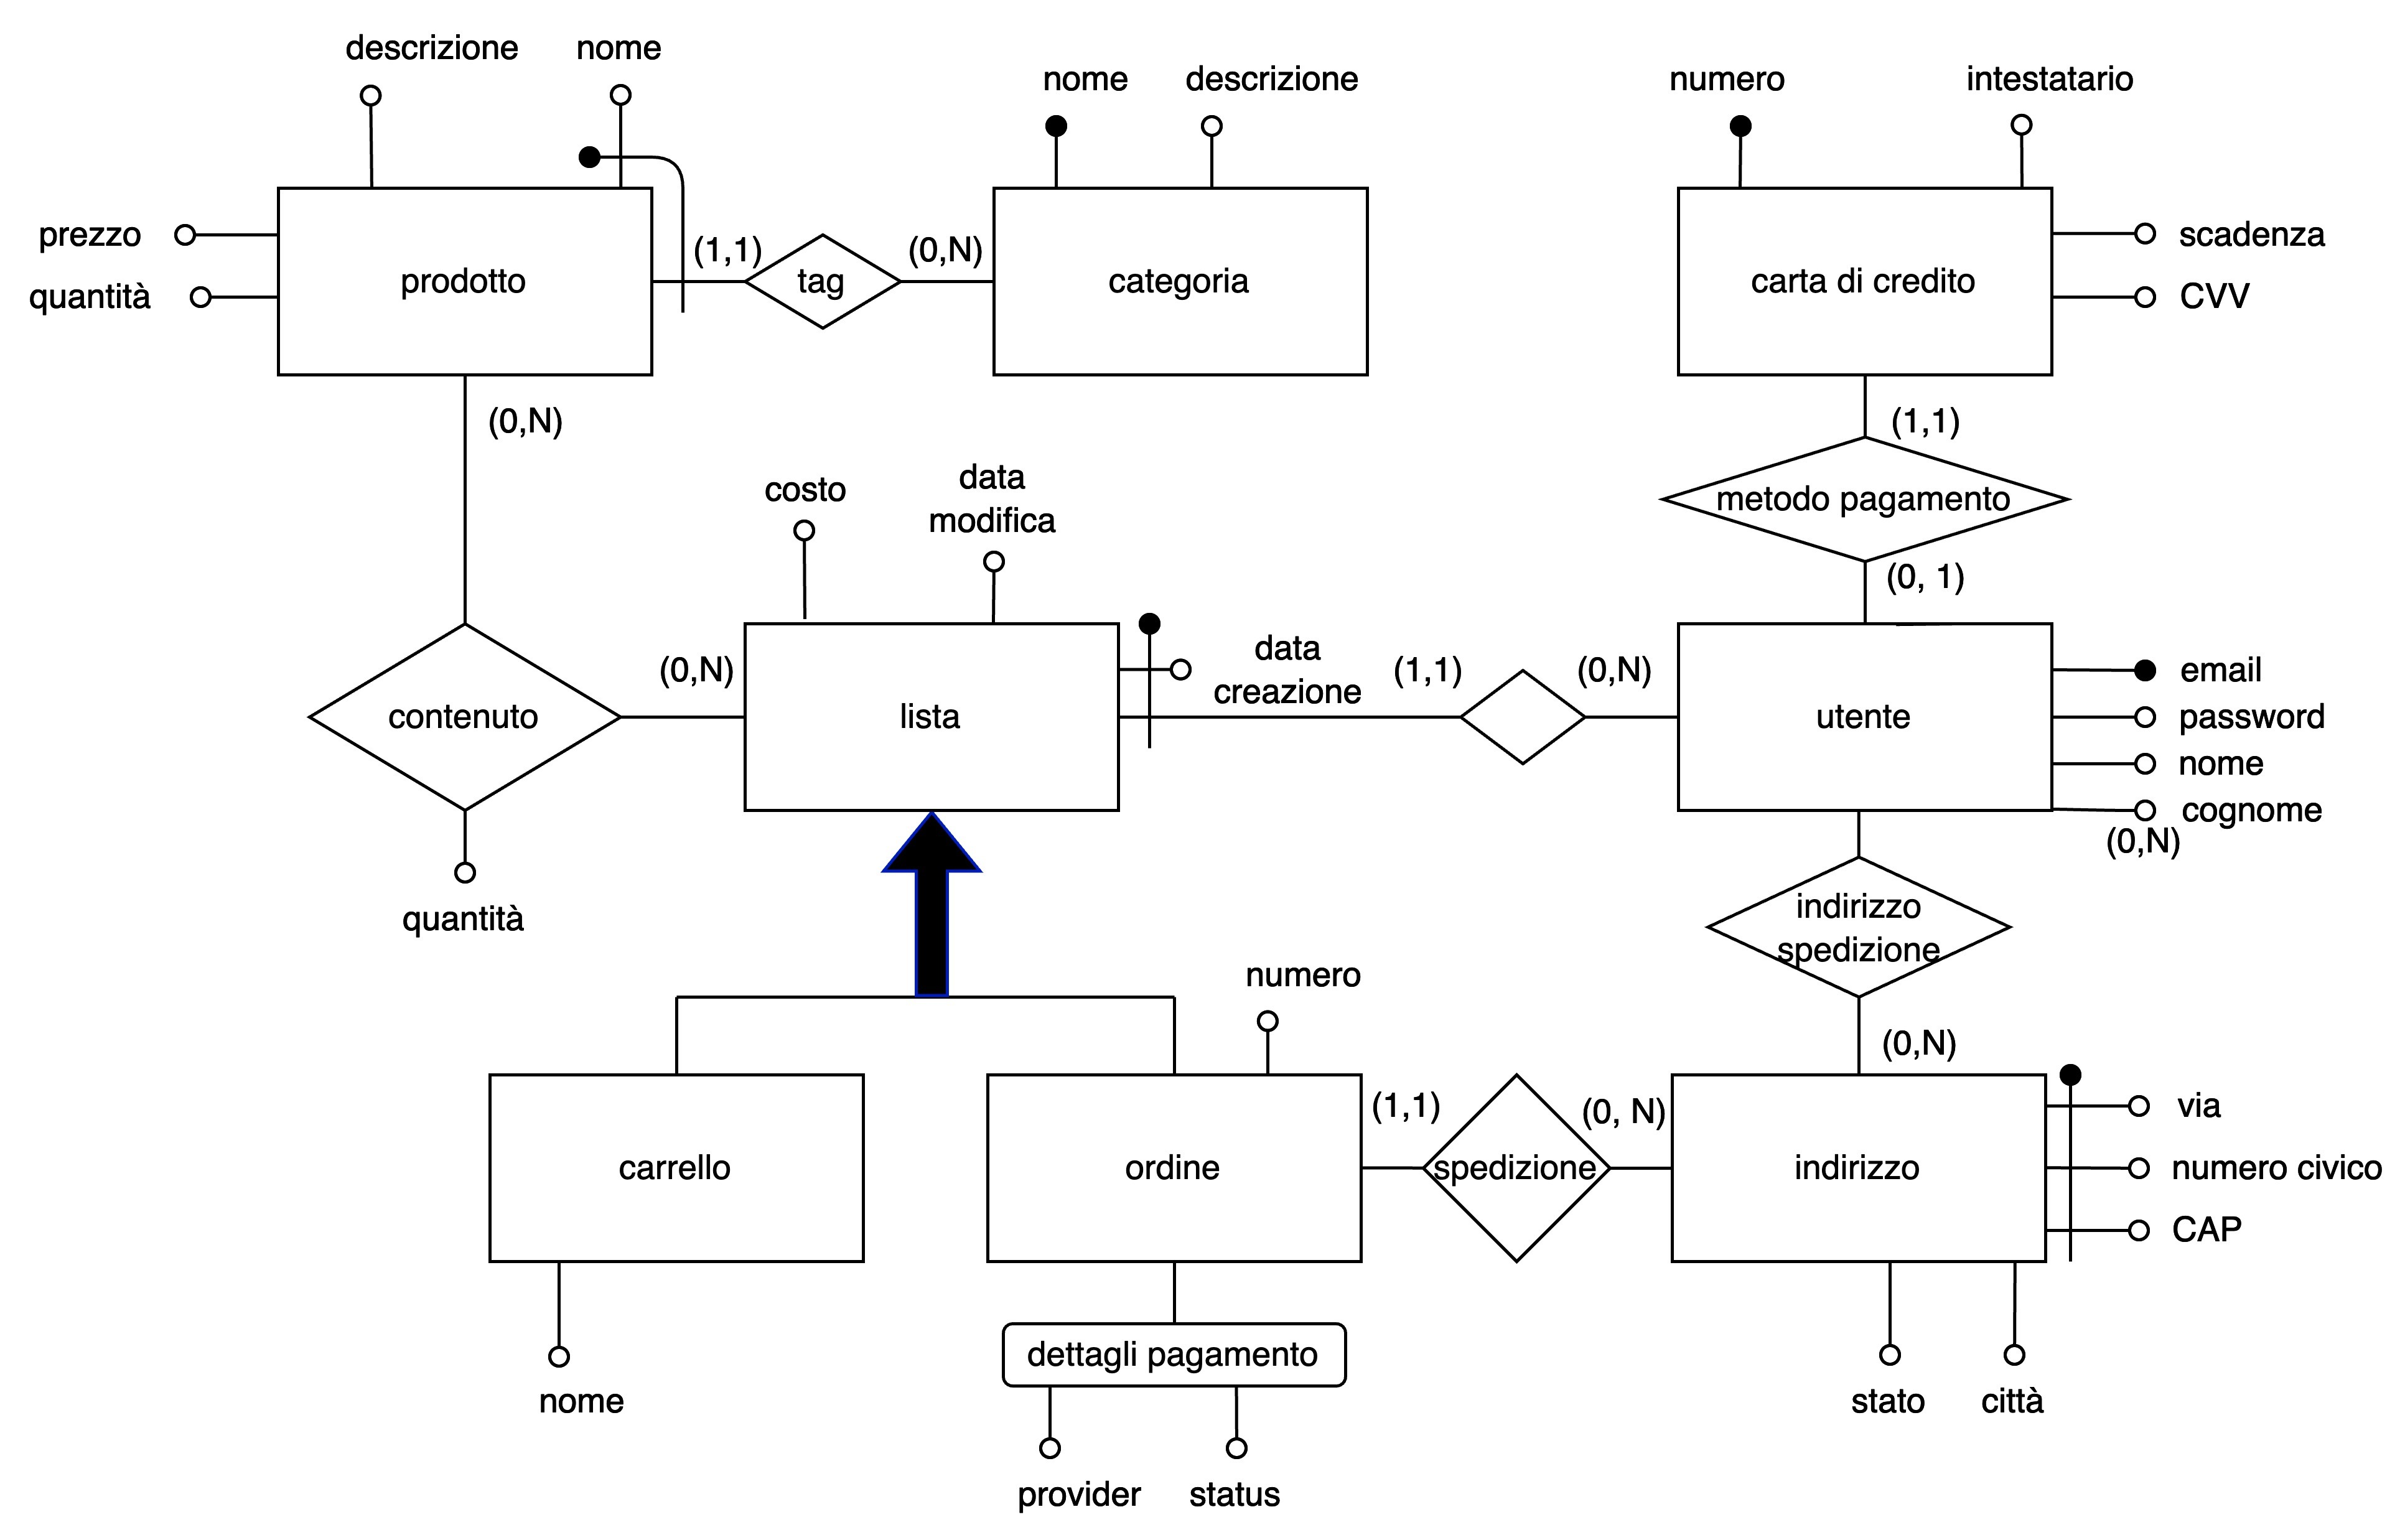
\includegraphics[width=\textwidth]{schema_concettuale}
	\caption{Schema concettuale}
\end{figure}

\section{Progettazione logica}

\subsection{Ristrutturazione}

\subsubsection{Analisi delle ridondanze}

L'attributo "Costo" dell'entità Lista è ridondante, in quanto può essere
calcolato come somma dei prezzi dei prodotti contenuti nella lista moltiplicati
per la quantità di ciascuno di essi. L'attributo "Costo" viene utilizzato nelle
operazioni:
\begin{enumerate}
	\item Aggiungi Prodotto al Carrello
	\item Rimuovi Prodotto dal Carrello
	\item Visualizza Carrello
	\item Visualizza Ordine
\end{enumerate}

Poichè le operazioni 1 e 2 modificano l'attributo "Costo" dell'entità Lista e
entrambe queste due operazioni sono molto più frequenti dell'operazione 3, si
toglie l'attributo "Costo" dall'entità Lista e si calcola il costo della lista
ogni volta che viene richiesta l'operazione 3. Si potrebbe pensare di aggiungere
l'attributo "Costo" all'entità Ordine, ma l'operazione 4 è poco frequente.

\begin{table}[H]
	\centering
	\begin{tabularx}{\textwidth}{|l|X|}
		\hline
		\textbf{Generalizzazione} & \textbf{Risoluzione} \\
		\hline
		Lista $\leftarrow$ Carrello, Ordine & L'entità Carrello è accorpata in
		Lista, con l'aggiunta di un attributo "nome VARCHAR(255) not null".
		L'entità Ordine è rappresentata mediante una relazione tra Lista (0,1) e
		Indirizzo (0, N), dove gli attributi di Ordine diventano attributi della
		relazione. \\
		\hline
	\end{tabularx}
	\caption{Eliminazione delle generalizzazioni}
\end{table}

\subsubsection{Scelta degli identificatori primari}
È stato introdotto l'attributo "ID" per le entità Prodotto, Indirizzo e Lista, 
dunque è stato rimosso l'attributo "Numero" dall'entità Ordine.


\begin{figure}[H]
	\centering
	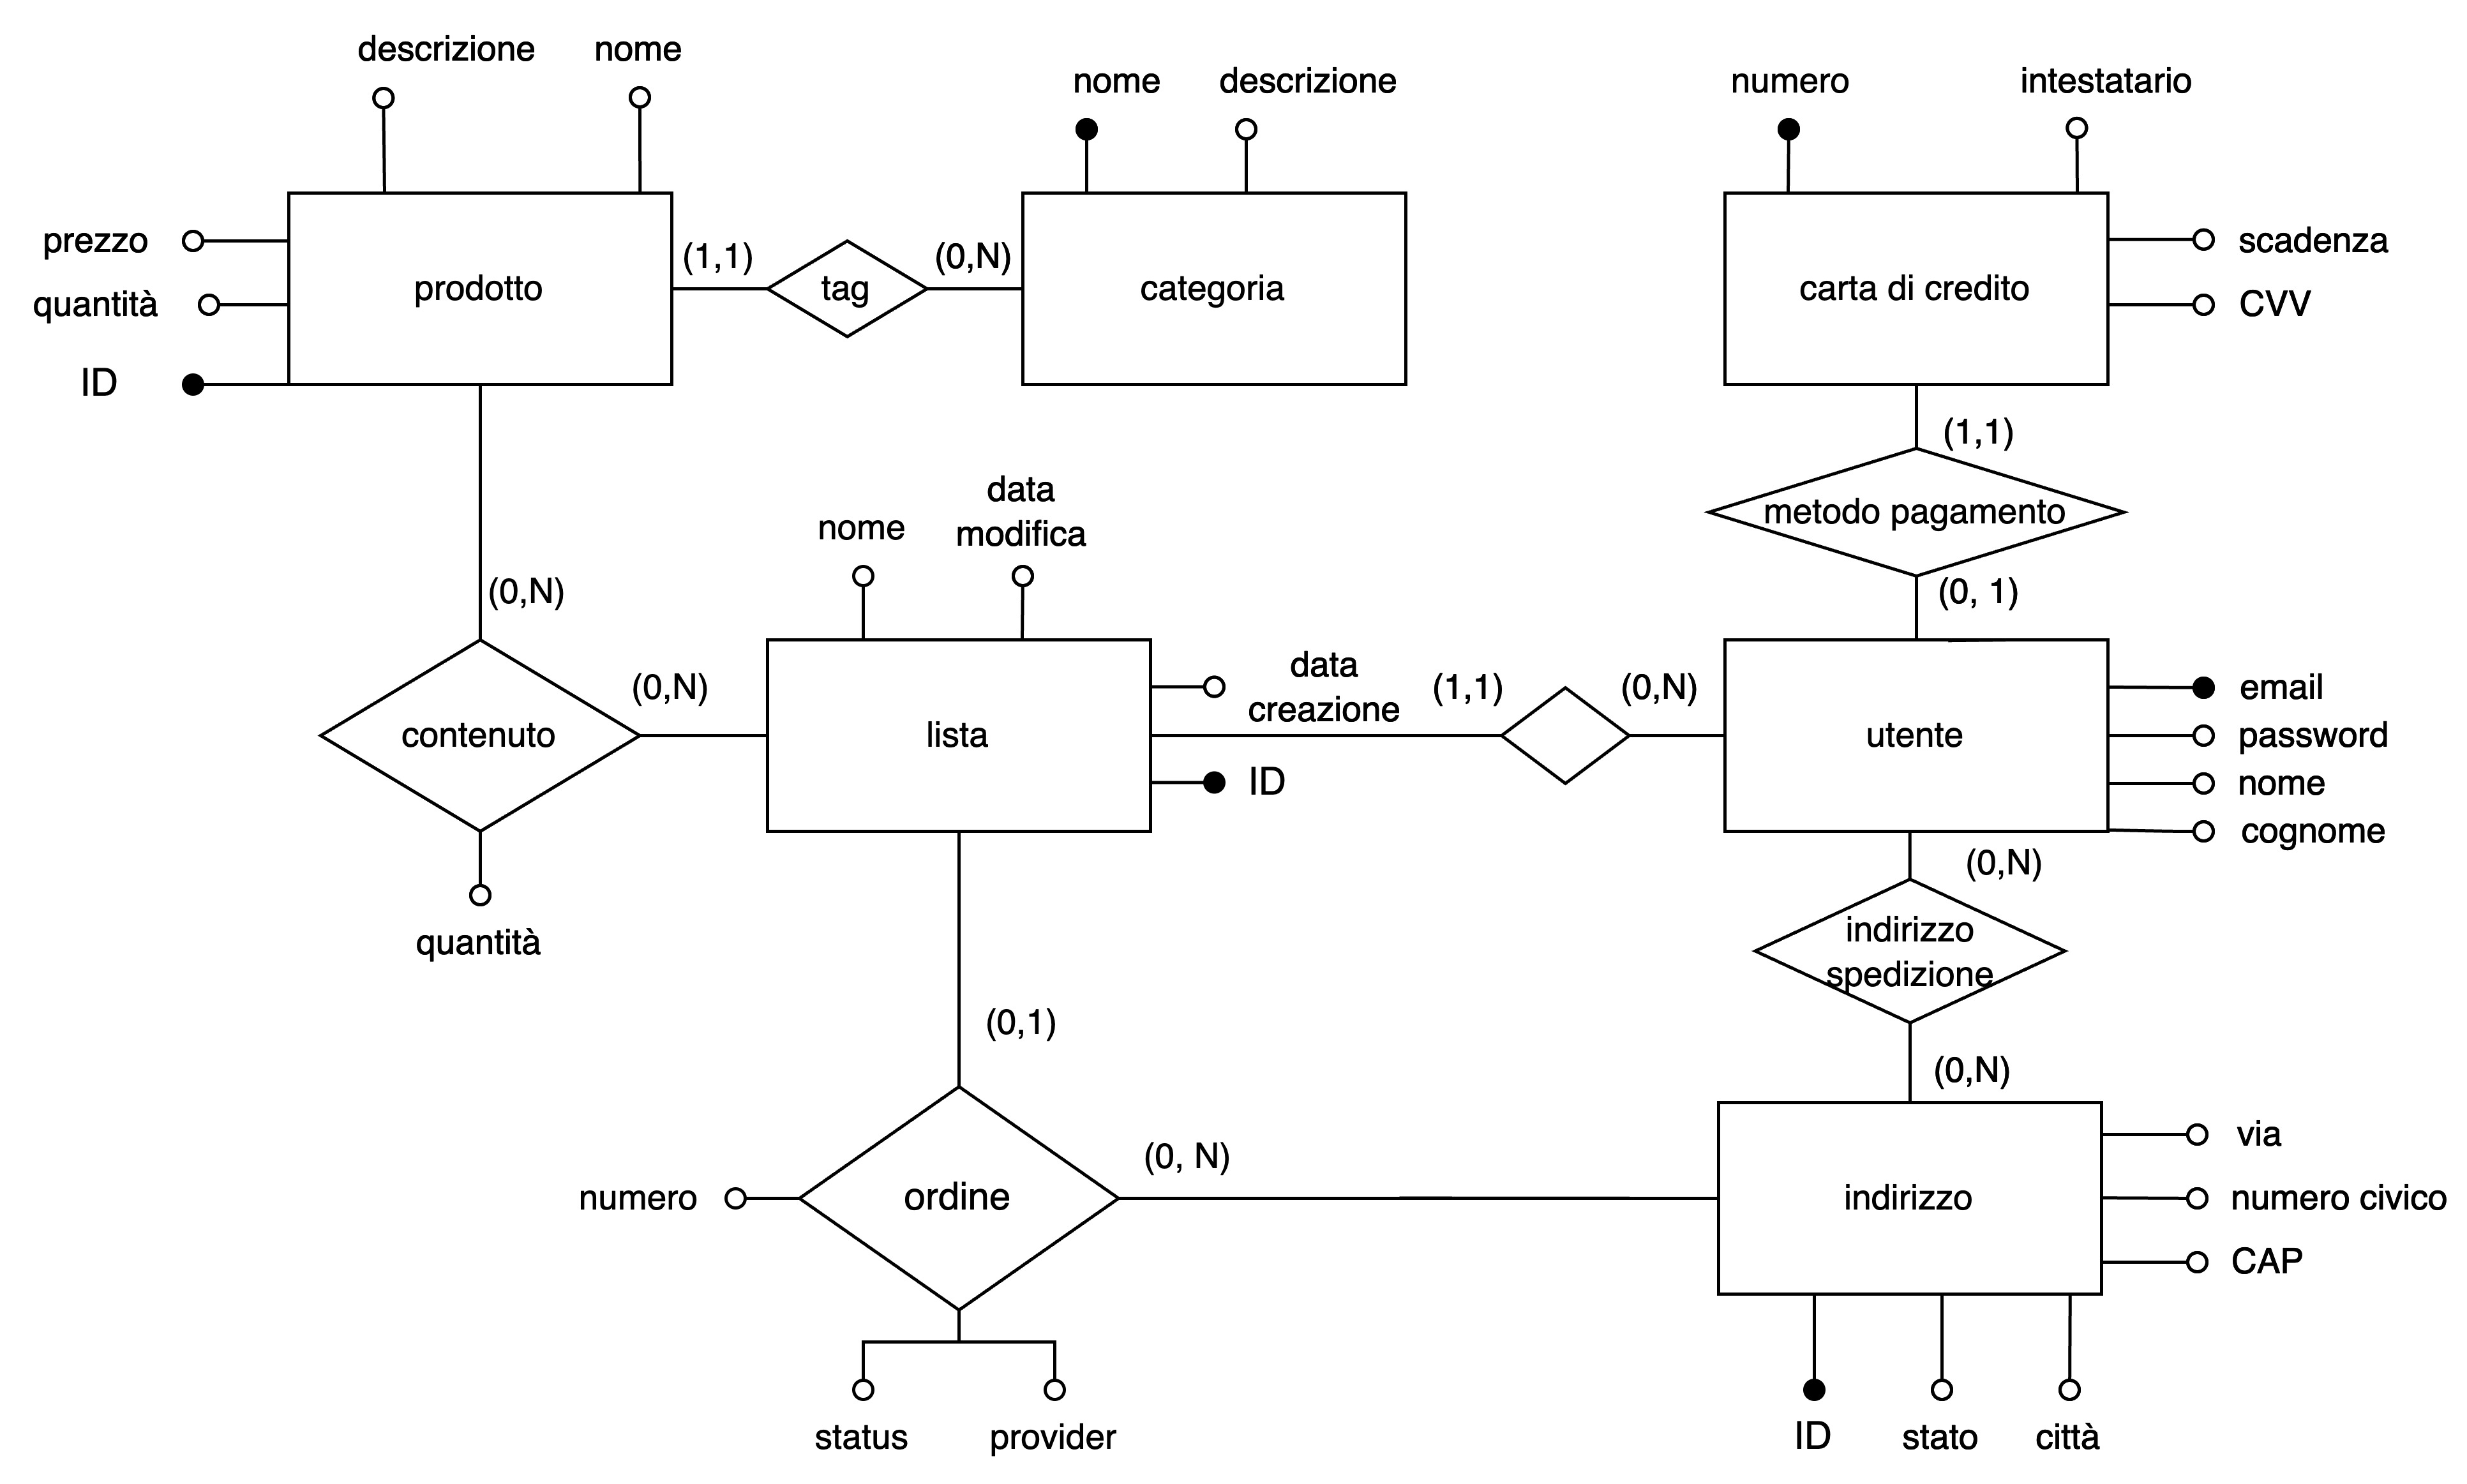
\includegraphics[width=\textwidth]{schema_logico}
	\caption{Schema E-R ristrutturato}
\end{figure}

\subsubsection{Creazione delle tabelle}
$A \rightarrow B$ indica che B è chiave esterna di A.

\paragraph{Carta di credito}(\underline{numero}, intestatario, scadenza,
CVV, utente $\rightarrow$ Utente.email)

\paragraph{Utente}(\underline{email}, password, nome, cognome)

\paragraph{Indirizzo spedizione}(\underline{utente} $\rightarrow$ Utente.email,
\underline{indirizzo} $\rightarrow$ Indirizzo.ID)

\paragraph{Indirizzo}(\underline{ID}, via, numero civico, CAP, città, stato)

\paragraph{Ordine}(\underline{lista} $\rightarrow$ Lista.ID, 
indirizzo $\rightarrow$ Indirizzo.ID, status, provider)

\paragraph{Lista}(\underline{ID}, nome, utente $\rightarrow$ Utente.email, data
creazione, data modifica)

\paragraph{Contenuto}(\underline{lista} $\rightarrow$ Lista.ID,
\underline{prodotto} $\rightarrow$ Prodotto.ID, quantità)

\paragraph{Prodotto}(\underline{ID}, nome, descrizione, prezzo, quantità, tag
$\rightarrow$ Categoria.nome)

\paragraph{Categoria}(\underline{nome}, descrizione)

\section{Here I write the queries}

\begin{lstlisting}[language=SQL]
SELECT lista.utente, sum(contenuto.quantita)
FROM lista, contenuto
WHERE lista.id = contenuto.lista 
AND lista.data_creazione > '2023-01-01'
GROUP BY (lista.utente);
\end{lstlisting}





\begin{lstlisting}[language=SQL]
SELECT utente.email, count(utente.email)
FROM utente, lista, ordine
WHERE utente.email = lista.utente
AND lista.id = ordine.lista
GROUP BY (utente.email)
\end{lstlisting}




\begin{lstlisting}[language=SQL]
SELECT email, count(email) 
FROM ((
	SELECT utente.email, lista.id from utente, lista
	WHERE utente.email = lista.utente) as tab
	LEFT OUTER JOIN ordine
	ON tab.id = ordine.lista)
WHERE lista IS NULL
GROUP BY email
\end{lstlisting}




\begin{lstlisting}[language=SQL]
SELECT ordine.lista, 
	sum(prodotto.prezzo * contenuto.quantita) as totale
FROM ordine, prodotto, contenuto
WHERE ordine.lista = contenuto.lista
AND prodotto.id = contenuto.prodotto
GROUP BY ordine.lista
\end{lstlisting}




\begin{lstlisting}[language=SQL]
SELECT lista.nome, totale 
FROM (
	SELECT tab.id, sum(prezzo * quantita) as totale
	FROM (
		SELECT lista.id as id, prodotto.prezzo, 
			contenuto.quantita
		FROM lista, prodotto, contenuto
		WHERE lista.id = contenuto.lista
		AND prodotto.id = contenuto.prodotto
	) as tab 
	LEFT JOIN ordine
	ON tab.id = lista
	WHERE indirizzo is NULL
	GROUP BY tab.id) as tab2, lista
WHERE tab2.id = lista.id;
\end{lstlisting}




\begin{lstlisting}[language=SQL]
SELECT DATE(data_creazione) AS day, sum(totale)
FROM lista, (
	SELECT ordine.lista, 
		sum(prodotto.prezzo * contenuto.quantita) AS totale
	FROM ordine, prodotto, contenuto
	WHERE ordine.lista = contenuto.lista
	AND prodotto.id = contenuto.prodotto
	GROUP BY ordine.lista) as costo_ordini
WHERE lista.id = lista
GROUP BY day;
\end{lstlisting}





\begin{lstlisting}[language=SQL]
SELECT EXTRACT(YEAR from data_creazione) AS year, 
	EXTRACT(MONTH from data_creazione) AS month, sum(totale)
FROM lista, (
	SELECT ordine.lista, 
		sum(prodotto.prezzo * contenuto.quantita) AS totale
	FROM ordine, prodotto, contenuto
	WHERE ordine.lista = contenuto.lista
	AND prodotto.id = contenuto.prodotto
	GROUP BY ordine.lista) AS costo_ordini
WHERE lista.id = lista
GROUP BY year, month
ORDER BY year, month;
\end{lstlisting}





\begin{lstlisting}[language=SQL]
SELECT p.tag, sum(p.prezzo * c.quantita) as totale
FROM prodotto as p, contenuto as c, ordine as o
WHERE p.id = c.prodotto
AND o.lista = c.lista
GROUP BY p.tag
HAVING sum(p.prezzo * c.quantita) > 100
ORDER BY totale DESC;
\end{lstlisting}


\end{document}
